\appendix
\section{Triplet Generation}

We attempted to generate Head, Relation, Tail (\(<H> <R> <T>\)) triplets following the model proposed in BloSum \cite{bhushan-lee-2022-block}.

\begin{figure}[h]
    \centering
    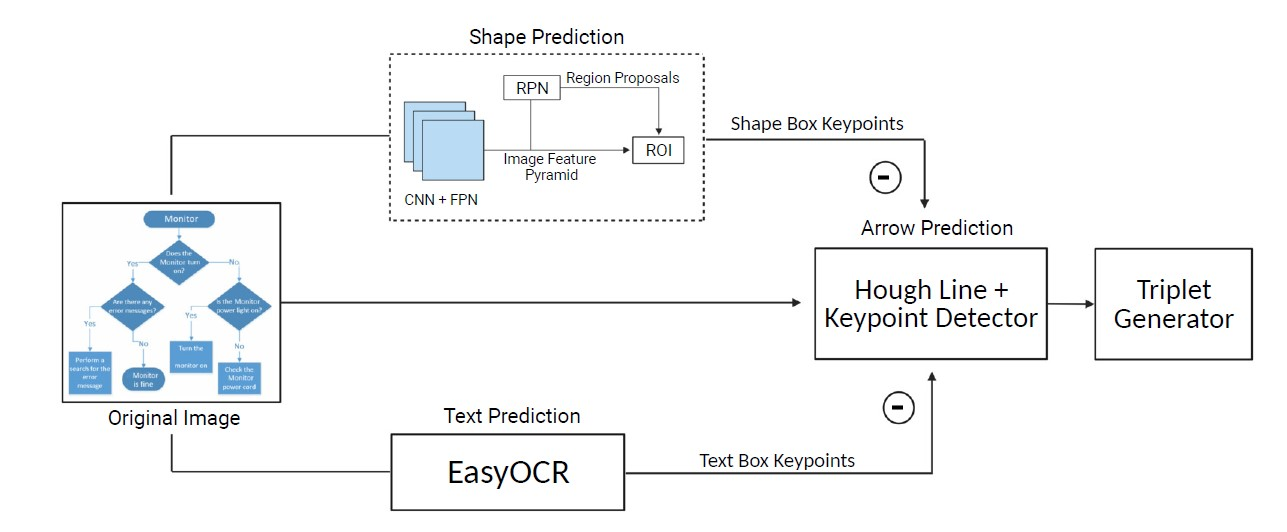
\includegraphics[width=0.48\textwidth]{Images/Triplet architecture.jpg} 
    \caption{Overall Architecture proposed in BloSum}
    \label{fig:appendix_triplet_architecture}
\end{figure}

\subsection{Text Prediction}

We used EasyOCR (Jaided, 2020) for detecting text \(T\) in an image. For each text \(t \in T\), it predicts a bounding box \(b_t \in \mathbb{R}^4\). We combined texts \(t\) where \(t\)'s bounding box falls within the bounding box of a shape \(s\).

\begin{figure}[h]
    \centering
    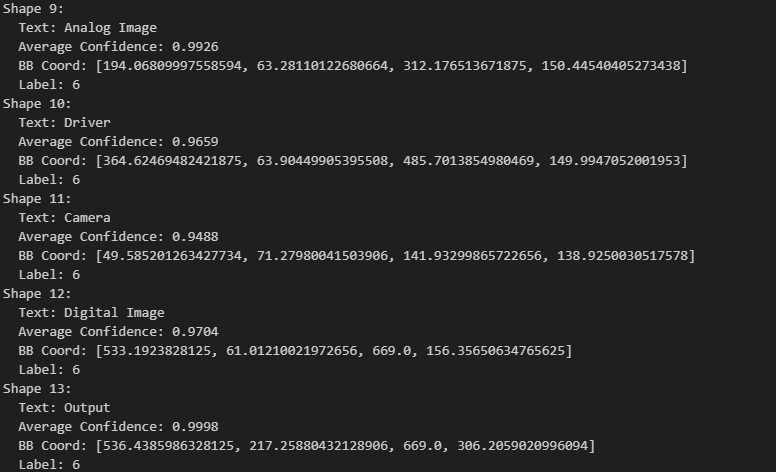
\includegraphics[width=0.48\textwidth]{Images/Sample output for easyOCR.jpg} 
    \caption{Sample Output for EasyOCR}
    \label{fig:appendix_isolated}
\end{figure}

\subsection{Arrow Prediction}

We subtracted non-arrow classes from the image before binarizing it to leave only the arrows behind. We then applied the Hough Line Transform to detect break and connecting arrows. We predicted the head and tail of an arrow by counting white pixels at the start and end points.

\begin{figure}[h]
    \centering
    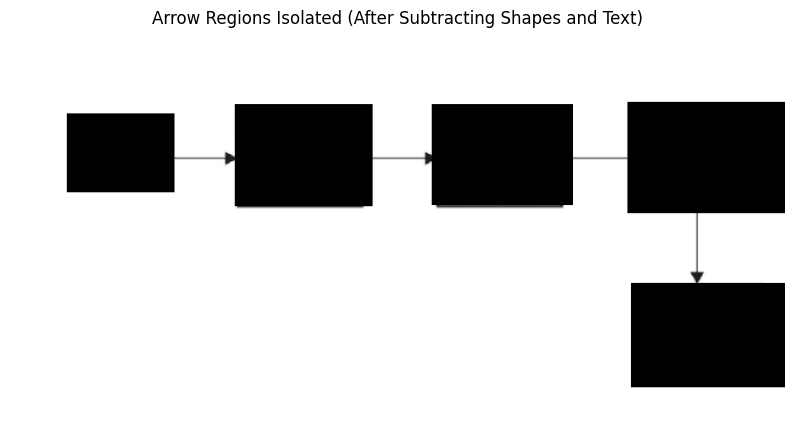
\includegraphics[width=0.48\textwidth]{Images/isolated.png} 
    \caption{Image after subtracting non-arrow classes}
    \label{fig:appendix_isolated}
\end{figure}

\begin{figure}[h]
    \centering
    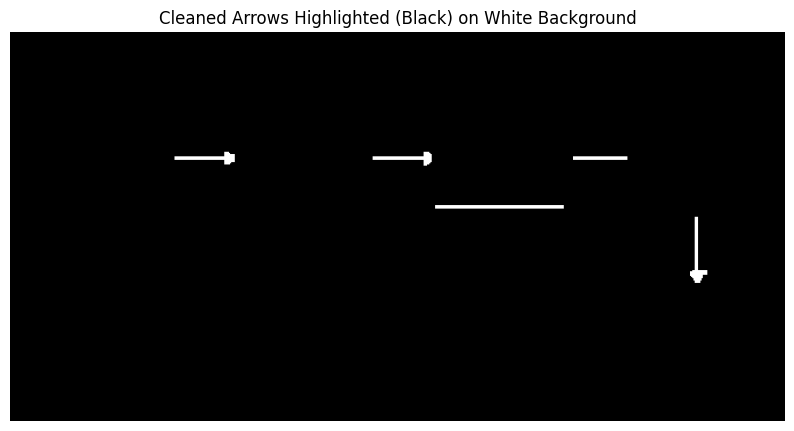
\includegraphics[width=0.48\textwidth]{Images/Binarized.png} 
    \caption{Image after Binarization}
    \label{fig:appendix_binarized}
\end{figure}

\subsection{Triplet Generator Logic}

We attempted to apply the same triplet generator logic used in BloSum \cite{bhushan-lee-2022-block}.

\begin{figure}[h]
    \centering
    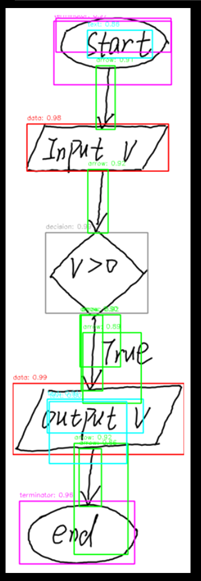
\includegraphics[width=0.48\textwidth]{Images/Fig Swin T CBD 50 epoch.png} 
    \caption{Fig Swin T CBD 50 epoch}
    \label{fig:appendix_binarized1}
\end{figure}

\begin{figure}[h]
    \centering
    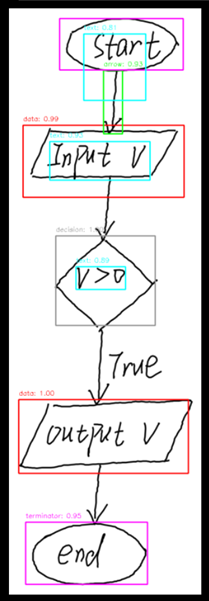
\includegraphics[width=0.48\textwidth]{Images/Swin t 100 epoch fca.png} 
    \caption{Swin t 100 epoch fca}
    \label{fig:appendix_binarized2}
\end{figure}

\begin{figure}[h]
    \centering
    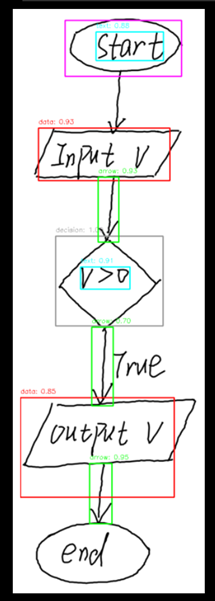
\includegraphics[width=0.48\textwidth]{Images/Inception Resnet 50 epochs.png} 
    \caption{Inception Resnet 50 epochs}
    \label{fig:appendix_binarized3}
\end{figure}



